\documentclass{article}

\usepackage[final]{assets/config}

\usepackage[utf8]{inputenc}
\usepackage[T1]{fontenc}

\usepackage[portuguese]{babel}

\usepackage{hyperref}
\usepackage{url}
\usepackage{booktabs}
\usepackage{amsfonts}
\usepackage{nicefrac}
\usepackage{microtype}
\usepackage{graphicx}

\usepackage{biblatex}
\addbibresource{referencial/referencias.bib}

\title{Relatório de Projeto Prático}

\author{
  Autor 1 \\
  Unidade de Engenharia e Computação \\
  Centro Universitário FAESA \\
  \texttt{autor1@email.com} \\
  \And
  Autor 2 \\
  Unidade de Engenharia e Computação \\
  Centro Universitário FAESA \\
  \texttt{autor2@email.com} \\
  \And
  Autor 3 \\
  Unidade de Engenharia e Computação \\
  Centro Universitário FAESA\\
  \texttt{autor3@email.com} \\
  \And
  Autor 4 \\
  Unidade de Engenharia e Computação \\
  Centro Universitário FAESA\\
  \texttt{autor4@email.com} \\
}

\begin{document}

\noindent\begin{minipage}{0.15\textwidth}

\includegraphics[width=2.0cm]{imagens/logo_faesa_pb.png}
\end{minipage}
\hfill
\begin{minipage}{1\textwidth}\raggedright
Centro Universitário FAESA \\
Eletrônica Básica I \\
\end{minipage}

\maketitle

\begin{abstract}
  Faça aqui uma breve apresentação de seu relatório. Insira uma pequena contextualização, quais os objetivos a serem alcançados, o método utilizado e os resultados alcançados.
\end{abstract}

\section{Introdução}

Inserir aqui uma breve introdução do trabalho, qual a motivação do desenvolvimento do relatório, a descrição do trabalho realizado e demais informações sobre o projeto.

\section{Trabalhos correlatos / Background teórico}

Nesta seção, inserir, se necessário, trabalhos correlatos que ajudem na sua argumentação teórica. Fique a vontade para inserir, também, referências bibliográficas, devidamente documentadas no capítulo de referências, para encorpar o seu trabalho \cite{teste}.

\section{Metodologia de Trabalho}

Inserir nesta seção as etapas metodológicas para o desenvolvimento do trabalho. Alguns exemplos de etapas metodológicas podem ser:

\begin{itemize}
    \item Revisão bibliográfica para o desenvolvimento do trabalho;
    \item Experimentação empírica e montagem do circuito;
    \item Cálculo dos parâmetros do projeto;
    \item Confecção do relatório prático da disciplina.
\end{itemize}

\section{Resultados}

Nesta seção, deverão ser apresentados os resultados do trabalho realizado. Vocês podem inserir imagens no trabalho, conforme o código abaixo:

\begin{figure}[htp]
    \centering
    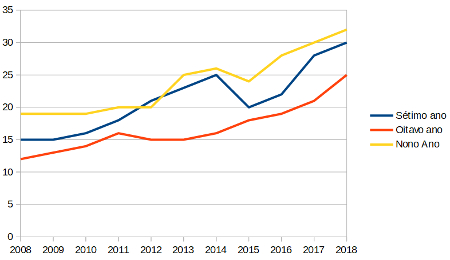
\includegraphics[width=10cm]{imagens/grafico.jpg}
    \caption{Um gráfico como exemplo.}
    \label{fig:galaxy}
\end{figure}

Vocês também podem trabalhar com equações matemáticas com bastante destreza no Latex.

\[ x^n + y^n = z^n \]

Podemos trabalhar, obviamente, com expressões um pouco mais cabulosas:

$$\lim_{x\to\infty} f(x)$$

$$\sum_{n=1}^{\infty} 2^{-n} = 1$$	

$$\oint_V f(s) \,ds$$

Apesar de um pouco complexo, é possível trabalhar com tabelas no Latex, como pode-se ver com o código a seguir:

\begin{tabular}{ |p{3cm}||p{3cm}|p{3cm}|p{3cm}|  }
 \hline
 \multicolumn{4}{|c|}{Lista de Países} \\
 \hline
 Nome do País ou Área& Código ISO Alpha 2 & Código Alpha 3& Código Numérico Alpha\\
 \hline
 Afghanistan   & AF    &AFG&   004\\
 Aland Islands&   AX  & ALA   &248\\
 Albania &AL & ALB&  008\\
 Algeria    &DZ & DZA&  012\\
 American Samoa&   AS  & ASM&016\\
 Andorra& AD  & AND   &020\\
 Angola& AO  & AGO&024\\
 \hline
\end{tabular}

Para conhecer um pouco mais sobre as funcionalidades do ambiente, não deixe de acessar a documentação em \url{https://www.overleaf.com/learn/latex/Main_Page}.


\section{Discussão e Análise dos Resultados}

Nesta seção é importante apresentar uma análise dos resultados encontrados. Eles fazem sentido? Como você explica os resultados esperados? Se não forem os resultados esperados, quais os fatores que podem ter influenciado os resultados encontrados.


\section{Considerações Finais}

Insira aqui as considerações finais do relatório. Pense, para este tópico, nos seguintes itens:

\begin{itemize}
    \item Os objetivos do projeto foram alcançados?
    \item Quais as dificuldades encontradas no projeto?
    \item O que vocês fariam diferente?
    \item Quais as contribuições deste projeto para a formação de vocês?
    \item Todos os membros do grupo trabalharam igualmente?
\end{itemize}

\printbibliography

\end{document}
